\chapter{Results and Discussion}
\label{chap:evaluation}

\section{Relations of Parliament Clubs}
\label{sec:relations_clubs}

\begin{figure}
\begin{tabular}{ l r}
	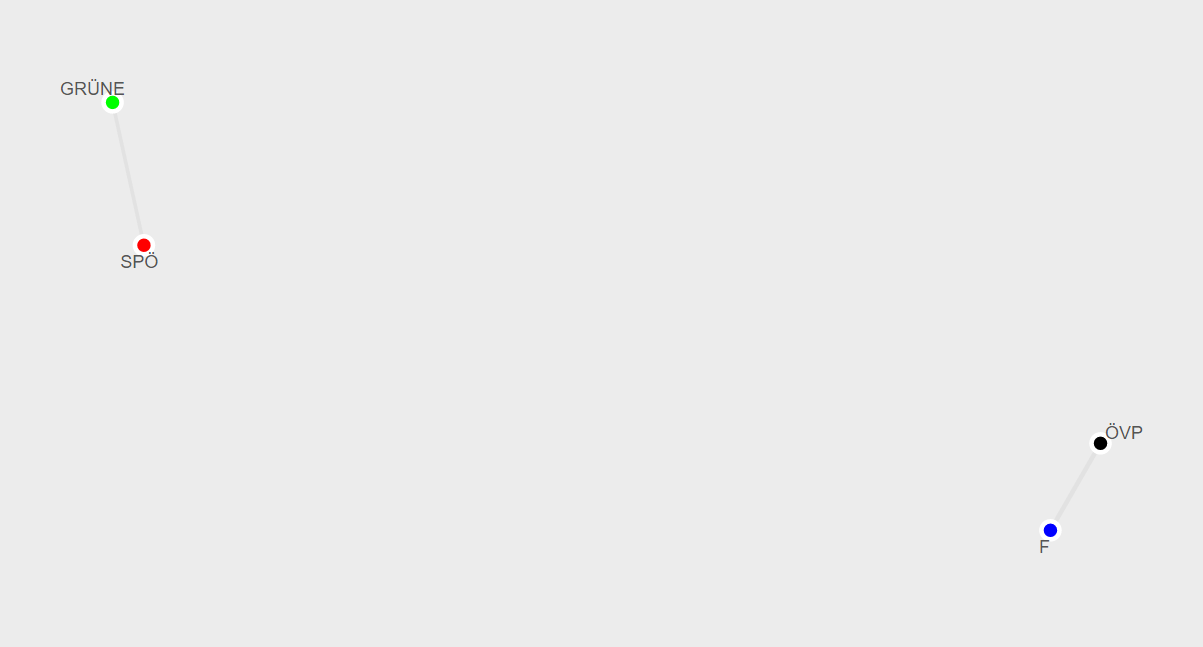
\includegraphics[width=0.49\textwidth]{imgs/graphs/club-graphs/clubs_21} & 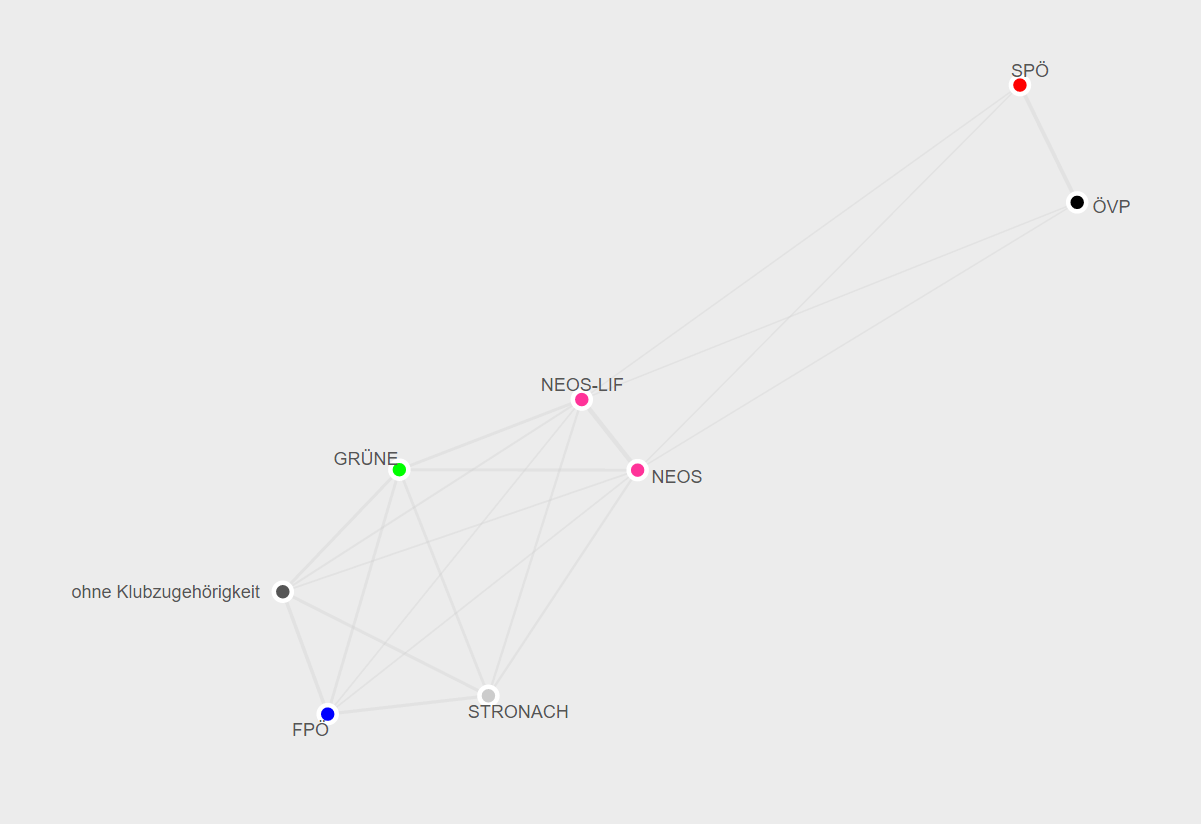
\includegraphics[width=0.49\textwidth]{imgs/graphs/club-graphs/clubs_25}
\end{tabular}
	\caption{Club ............}
	\label{fig:club_graphs1}
\end{figure}


\section{Relations of Politicians}
Graph + Explanations

\section{Government - Opposition Relation}
\label{sec:gov_opp_relation}

\begin{table}[h]

\bgroup
\def\arraystretch{1.2}
\begin{tabular}{| l | l | p{4cm} | l |}
\hline
  Legislative Period & Governing Parties & Opposition & \linebreakcell{Relationship\\Coefficient}  \\
\hline
\hline
  XX. Period & SPÖ, ÖVP & FPÖ, Grüne, Liberale & -0.85 \\
\hline
  XXI. Period & ÖVP, FÖP & SPÖ, Grüne & -0.695 \\
\hline
  XXII. Period & ÖVP, FPÖ, BZÖ & SPÖ, Grüne & -0.567 \\
\hline
  XXIII. Period & SPÖ, ÖVP & FPÖ, Grüne, BZÖ & -0.382 \\
\hline
  XXIV. Period & SPÖ, ÖVP & FPÖ, Grüne, Stronach, BZÖ & -0.52 \\
\hline
  XXV. Period & SPÖ, ÖVP & FPÖ, Grüne, NEOS, Stronach & -0.374 \\
\hline

\end{tabular}
\egroup
\caption{Relation of Government and Opposition in the periods 20 to 25}
\label{table:gov_opp_relation}
\end{table}